\documentclass[acmsmall,screen,review]{acmart}
\usepackage{algorithm}
\usepackage{algpseudocode}
\usepackage{booktabs}
\usepackage{multirow}
\usepackage{listings}
\usepackage{xcolor}
\usepackage{amsmath}
\usepackage[capitalize]{cleveref}
\usepackage{xspace}
\usepackage{xurl}
\usepackage{tikz}
\usetikzlibrary{arrows.meta,positioning,shapes.geometric}
\newcommand{\tool}{\textsc{kfold}\xspace}
\newcommand{\kmax}{\textsc{Kmax}\xspace}

\AtBeginDocument{%
  \providecommand\BibTeX{{Bib\TeX}}}

\setcopyright{none}
\settopmatter{printacmref=false}

\lstset{
  basicstyle=\ttfamily\footnotesize,
  keywordstyle=\bfseries\color{blue!70!black},
  commentstyle=\itshape\color{green!50!black},
  stringstyle=\color{red!60!black},
  breaklines=true,
  numbers=left,
  numberstyle=\tiny\color{gray},
  stepnumber=1,
  numbersep=5pt,
  frame=single,
  tabsize=2
}

\begin{document}

\title{\tool: Scalable and Exact Object-Selection Conditions for Kbuild Makefiles}

\author{Anonymous Author(s)}
\affiliation{%
  \institution{Anonymous Institution}
  \country{USA}
}

\begin{abstract}
Kbuild Makefiles decide which objects enter the build of Linux and other configurable systems. A maintainer who asks why a file was not compiled, or which options would compile it, needs the option condition under which each object is built, but running Make reveals only the objects of one configuration. Computing these conditions statically requires following assignments whose destination depends on an option, overwrites that apply in only some configurations, composite objects, included fragments, directories reached along several paths, and objects that Kbuild builds only because a rule needs them. Executing a Makefile symbolically with one state per branch combination does not scale: on a generated Makefile with 16 independent options, a forking executor tracks more than half a million states. We present \tool, which executes Kbuild Makefiles with a Boolean guard on every word of every variable. Appends add guarded words, a conditional overwrite re-guards the words it replaces, and the two arms of a conditional merge into one state at \texttt{endif}, so the state stays linear in the number of words. A directory worklist propagates to each Makefile only the part of an incoming guard not already covered, and a closure over rules adds the objects that selected files depend on.

We evaluate \tool on Linux v6.6 and four other Kbuild-based systems by evaluating its conditions under concrete configurations and comparing the predictions with the objects of real builds and with GNU Make's own expansion of each Makefile. On four Linux configurations, from \texttt{tinyconfig} to \texttt{allmodconfig}, \tool's predicted objects are exactly the compiled objects: 489 to 25,949 objects, with no false positive and no miss. Per Makefile, its target lists match GNU Make for all 922 to 12,605 active targets. \tool analyzes the 2,022 Makefile instances of the Linux x86 tree in 34\,s and 162\,MB, and its time stays flat on generated Makefiles where the forking executor times out. These results show that per-word guards, together with a faithful model of Kbuild's build semantics, yield object-selection conditions that are both scalable and exact at kernel scale.
\end{abstract}

\begin{CCSXML}
<ccs2012><concept><concept_id>10011007.10011074.10011099.10011692</concept_id><concept_desc>Software and its engineering~Software verification</concept_desc><concept_significance>500</concept_significance></concept></ccs2012>
\end{CCSXML}
\ccsdesc[500]{Software and its engineering~Software verification}
\keywords{Kbuild, build systems, variability, symbolic execution, object selection}
\maketitle
\pagestyle{plain}

\section{Introduction}
\label{sec:intro}

The build system determines which source files reach the compiler. In the Linux kernel and related projects, Kbuild expresses this choice through Make variables such as \texttt{obj-\$(CONFIG\_USB)} and through conditionally selected subdirectories. A concrete build reveals the objects selected by one \texttt{.config}; it does not say which option settings would select a different object. A build condition for every object would let a maintainer explain why a source file was not compiled, compare build rules across releases, or search for a configuration that enables a given target. Analyses of configuration-dependent compilation errors and unmet dependencies already consume such conditions~\cite{gazzillo2018localizing,oh2021kclause,yildiran2021kismet}.

Recovering these conditions requires more than collecting the \texttt{CONFIG\_*} names that appear near an object. Consider two consecutive lines of a Kbuild Makefile:
\begin{center}
\texttt{obj-\$(CONFIG\_NET) += net\_core.o}\qquad\texttt{obj-\$(CONFIG\_FAST) := fast\_net.o}
\end{center}
The first line appends \texttt{net\_core.o} to \texttt{obj-y} when \texttt{CONFIG\_NET=y}. The second computes its destination from \texttt{CONFIG\_FAST}: when that option is \texttt{y}, it \emph{replaces} \texttt{obj-y}; otherwise it assigns an unselected variable such as \texttt{obj-} and leaves \texttt{obj-y} alone. The correct condition for \texttt{net\_core.o} is therefore $\texttt{CONFIG\_NET}\land\neg\texttt{CONFIG\_FAST}$. Further conditions come from \texttt{ifeq} blocks, from composite objects whose members are listed in other variables, from fragments included with \texttt{include}, from the chain of parent directories through which Kbuild reaches a Makefile, and from rules: the Linux boot image, real-mode trampoline, and vDSO consist of objects that no target list names and that Kbuild builds only because a rule needs them.

Symbolic execution is a natural way to compute such conditions, because it evaluates Make's assignments and expansions as written while tracking the configurations under which each result holds. Its classic form keeps one state per path. An earlier symbolic executor for Kbuild Makefiles~\cite{nguyen2020using} forks a state at each conditional and merges only identical paths. Kbuild Makefiles, however, consist largely of independent conditional assignments, and each one that changes a value can double the number of distinct states. On a generated Makefile with 16 independent \texttt{ifeq} blocks that each append to a helper list, that executor tracks 524,289 states and needs 185\,s and 1.7\,GB; with 20 blocks it does not finish within five minutes (\Cref{sec:eval:scale}). The Linux x86 tree has 2,022 Makefile instances with thousands of such assignments.

\tool starts from the observation that Kbuild object lists are used as \emph{sets}: an object is either in \texttt{obj-y} or it is not. \tool therefore attaches a guard to each word rather than keeping one state per configuration. In the example, \texttt{obj-y} holds \texttt{net\_core.o} under $\texttt{CONFIG\_NET}\land\neg\texttt{CONFIG\_FAST}$ and \texttt{fast\_net.o} under \texttt{CONFIG\_FAST}. A conditional overwrite conjoins the negation of its own guard onto the words it may replace. For an \texttt{ifeq} block, \tool executes each arm on a copy of the state and merges the copies at \texttt{endif}, so one state continues after every conditional and $k$ guarded appends yield $k$ guarded words. Across directories, a worklist records for each Makefile the disjunction of guards already propagated to it and processes only the uncovered part of a new guard. On top of this representation, \tool models the parts of Kbuild's build semantics that decide which object files exist: composite members, the rule that built-in objects need a built-in route to their directory, host and user programs, and a closure over rules and sub-makes.

A scalable representation is useful only if its conditions are right, and the strongest evidence for that is agreement with real builds. We therefore evaluate \tool's conditions under concrete configurations against two references: the \texttt{.o} files that a build of that configuration produces, and GNU Make's expansion of the target lists in each traversed Makefile. The subjects are Linux v6.6 under four configurations, BusyBox, coreboot, Barebox, and Das U-Boot. On all four Linux configurations, \tool's predicted set equals the set of compiled objects, from 489 objects for \texttt{tinyconfig} to 25,949 for \texttt{allmodconfig}. Per Makefile, its target lists agree with GNU Make on every one of 922 to 12,605 active targets. \tool analyzes the Linux x86 tree in 34\,s and 162\,MB. On the same tree, \kmax~\cite{gazzillo2017kmax}, a static analysis that also carries configuration conditions on values, needs 86 minutes, fails on three directories that exceed a 12\,GB memory limit, and misses up to 7,902 compiled objects that it extracts.

This paper makes the following contributions:
\begin{enumerate}
\item A per-word guarded representation of Make variables, with guarded append, conditional overwrite, and branch merge operations for Kbuild-style assignments with computed names, and an expansion that preserves Make's semantics for word lists, partially defined variables, substitution references, and deferred appends (\Cref{sec:design:assign,sec:design:expand,sec:design:merge}).
\item A conditional directory worklist that propagates only uncovered guards, static splicing of included fragments, and a model of Kbuild's build semantics, including built-in routes and a closure over rules and sub-makes (\Cref{sec:design:worklist,sec:design:include,sec:design:build}).
\item \tool, an implementation that supports the target families, composite objects, and top-level entry points of five Kbuild dialects, and a web interface for querying Linux conditions (\Cref{sec:design:targets,sec:implementation}).
\item An evaluation against physical builds and GNU Make on five systems, with exact agreement on four Linux configurations, a scalability comparison with a forking symbolic executor and with \kmax, and an ablation of each design element (\Cref{sec:eval}).
\end{enumerate}

\section{Overview}
\label{sec:overview}

\Cref{fig:pipeline} shows how \tool turns Kbuild files and project entry points into a formula for each object path. \tool first parses each Makefile, splices in the fragments it includes, and removes statements that cannot affect target variables or rules. It then executes the remaining statements over guarded variable values, propagates directory guards from parent to child Makefiles, and finally collects guarded object paths: targets, composite members, program objects, and the prerequisites that rules need. A separate evaluator substitutes a concrete configuration into the formulas and compares the predictions with observed objects. The next subsections follow one Makefile through these stages; \Cref{sec:design} generalizes each operation.

\begin{figure*}[t]
\centering
\resizebox{\textwidth}{!}{%
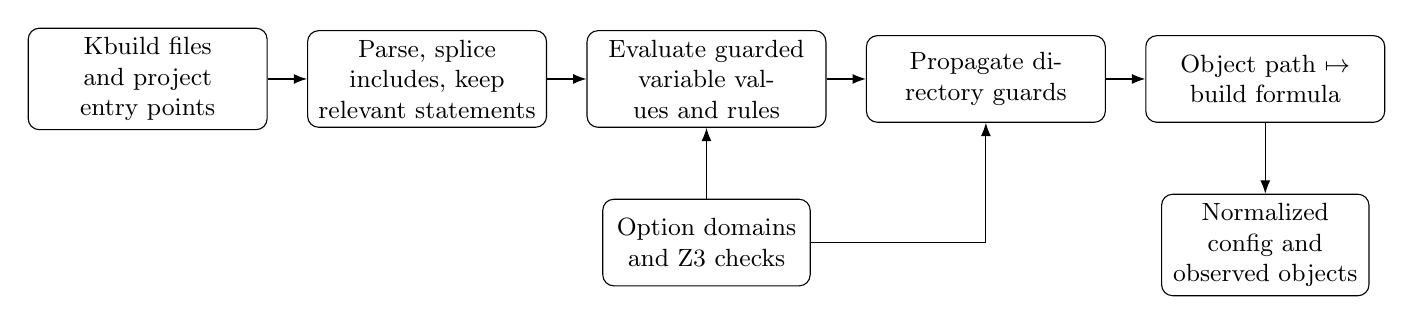
\begin{tikzpicture}[>=Latex, node distance=5mm and 5mm,
  box/.style={draw,rounded corners,align=center,minimum height=11mm,text width=28mm,font=\small},
  smallbox/.style={draw,rounded corners,align=center,minimum height=11mm,text width=24mm,font=\small}]
\node[box] (source) {Kbuild files and project entry points};
\node[box,right=of source] (parse) {Parse, splice includes, keep relevant statements};
\node[box,right=of parse] (execute) {Evaluate guarded variable values and rules};
\node[box,right=of execute] (walk) {Propagate directory guards};
\node[box,right=of walk] (output) {Object path $\mapsto$ build formula};
\draw[->] (source)--(parse);\draw[->] (parse)--(execute);\draw[->] (execute)--(walk);\draw[->] (walk)--(output);
\node[smallbox,below=9mm of execute] (domain) {Option domains and Z3 checks};
\draw[->] (domain)--(execute);\draw[->] (domain)-|(walk);
\node[smallbox,below=9mm of output] (concrete) {Normalized config and observed objects};
\draw[->] (output)--(concrete);
\end{tikzpicture}}
\caption{\tool computes one build formula per object path without choosing a configuration. A normalized configuration and the observed object inventory enter only afterward, to evaluate and validate the formulas.}
\Description{A five-stage flow from Kbuild files and entry points through parsing and include splicing, guarded-value evaluation, conditional directory traversal, and object build formulas. Option domains feed evaluation and traversal; a normalized configuration and observed objects enter only after extraction.}
\label{fig:pipeline}
\end{figure*}

\subsection{Kbuild selection in brief}
Kbuild uses GNU Make variables to describe objects. A line such as \texttt{obj-\$(CONFIG\_NET) += net.o} computes the destination variable name from an option. If the option expands to \texttt{y}, the word is appended to \texttt{obj-y} and linked into the kernel; \texttt{m} selects \texttt{obj-m} for a loadable module; an unset option produces \texttt{obj-}, which Kbuild ignores. A word ending in \texttt{/} asks Kbuild to descend into that subdirectory's Makefile. A target such as \texttt{driver.o} may be a composite assembled from the objects in \texttt{driver-y} or \texttt{driver-objs}, and a Makefile may pull further assignments from another file with \texttt{include}. The condition for an object therefore combines a local selection condition with a reachability condition inherited from its parent directories.

GNU Make also distinguishes immediate assignment with \texttt{:=} from deferred assignment with \texttt{=}. The former expands its right-hand side at assignment time; the latter stores an expression that is expanded when the variable is referenced. \texttt{+=} follows the variable's existing flavor, and \texttt{?=} assigns only when the variable is undefined. A reference to a variable that is not set in the current configuration expands to the empty string. These rules decide which assignment wins and what a reference produces, and so affect object lists even when a Makefile contains no explicit conditional.

\tool takes a source tree, per-project settings that name the entry directories and target-variable families, and a Boolean or tristate option domain. It outputs a set of object paths, each with a formula over those options.

\Cref{lst:example} is a simplified Kbuild Makefile that extends the two lines from \Cref{sec:intro}. It combines an assignment to a computed variable name, an overwrite, a conditional branch, and a composite target. For this example, assume that each option is either \texttt{y} or unset. We want a condition for each object, not a list for one chosen configuration.

\begin{lstlisting}[language=make,float=t,caption={Simplified Kbuild Makefile. Each object's final condition also includes the guard under which this directory is entered.},label={lst:example}]
obj-$(CONFIG_NET) += net_core.o
obj-$(CONFIG_FAST) := fast_net.o
ifeq ($(CONFIG_WIDE),y)
  WIDTH := 64
else
  WIDTH := 32
endif
obj-y += driver_$(WIDTH).o
fast_net-y += accelerator.o
\end{lstlisting}

\subsection{A trace from assignments to object conditions}
\label{sec:overview:trace}
\Cref{tab:example-trace} records the state after each statement of \Cref{lst:example}. We write $N$ for \texttt{CONFIG\_NET=y}, $F$ for \texttt{CONFIG\_FAST=y}, and $W$ for \texttt{CONFIG\_WIDE=y}. Line~1 adds one word, \texttt{net\_core.o}, with guard $N$. Line~2 assigns \texttt{obj-y} only when $F$ holds, so \tool adds \texttt{fast\_net.o} under $F$ and re-guards the existing word: \texttt{net\_core.o} survives under $N\land\neg F$. Treating the overwrite as unconditional would lose \texttt{net\_core.o}; ignoring it would keep \texttt{net\_core.o} under $N\land F$, where Make has replaced the value.

\begin{table}[t]
\centering\footnotesize
\caption{Guarded words after each statement of \Cref{lst:example}. The last column assumes that the directory is reached under guard $D$. The map records membership, not word order or multiplicity.}
\label{tab:example-trace}
\begin{tabular}{llll}
\toprule
Line & Step & State change & Final contribution \\
\midrule
1 & Append & \texttt{net\_core.o}: $N$ & $D\land N\land\neg F$ \\
2 & Conditional overwrite & \texttt{fast\_net.o}: $F$; \texttt{net\_core.o}: $N\land\neg F$ & $D\land F$ \\
3--7 & Conditional & \texttt{WIDTH}: \texttt{64} under $W$, \texttt{32} under $\neg W$ & --- \\
8 & Append & \texttt{driver\_64.o}: $W$ & $D\land W$ \\
8 & Append & \texttt{driver\_32.o}: $\neg W$ & $D\land\neg W$ \\
9 & Composite & \texttt{accelerator.o} belongs to \texttt{fast\_net.o} & $D\land F$ \\
\bottomrule
\end{tabular}
\end{table}

Lines~3--7 assign \texttt{WIDTH} in both arms of a conditional. \tool executes the then-arm on one copy of the state under $W$ and the else-arm on another under $\neg W$. At \texttt{endif}, it merges the copies: \texttt{WIDTH} holds \texttt{64} under $W$ and \texttt{32} under $\neg W$, and execution continues with one state. Line~8 expands \texttt{driver\_\$(WIDTH).o} into two words with complementary guards. Line~9 defines a composite: its parent \texttt{fast\_net.o} is selected under $F$, so its unconditional member \texttt{accelerator.o} inherits $F$. Finally, \tool conjoins every local condition with the guard $D$ under which the directory is reached, which gives the last column of \Cref{tab:example-trace}.

A forking executor would instead carry one environment for each combination of $N$, $F$, and $W$ that produces a different \texttt{obj-y}, and every further independent conditional that changes the list can double that number. \tool's state after line~9 holds five guarded object words, and a further independent append adds one more.

\subsection{The same object through two directories}
\label{sec:overview:directories}
Directory guards need the same care as variable guards. Suppose a root Makefile selects \texttt{a/} under option $A$ and \texttt{b/} under option $B$, and both directories select \texttt{shared/}. If \texttt{shared/Makefile} selects \texttt{x.o}, the condition for \texttt{x.o} is $A\lor B$. Marking \texttt{shared/} as visited after the $A$ path would lose the $B$ contribution. \tool instead records, for each Makefile, the disjunction of the guards already propagated to it. When $B$ arrives, it processes only $B\land\neg A$; if $A$ already covered $B$, it does no new work. For the same reason, a back edge from \texttt{shared/} to \texttt{a/} stops once it contributes no new configuration.

\section{Technique}
\label{sec:design}

\subsection{Setting and algorithm}
\label{sec:design:alg}
Let $M$ be a collection of Kbuild Makefiles and $c$ an assignment to the option symbols they use. For an object path $o$, write $S_M(o,c)$ when Kbuild builds $o$ under $c$. \tool computes a formula $\Phi_M(o)$ such that evaluating $\Phi_M(o)$ under $c$ predicts $S_M(o,c)$. A variable's state $\sigma[n]$ is a map from words to formulas: an entry $w\mapsto\phi$ says that $w$ belongs to variable $n$ in configurations satisfying $\phi$. We write $\sigma[n](w)=\bot$ for an absent word and $\sqcup$ for the pointwise disjunction of two such maps.

\Cref{alg:extract} gives the end-to-end procedure. Its input is the source tree, the entry Makefiles $E$ with their guards, and project settings $\Gamma$ that name target-variable families and option domains; its output is the map $\Phi$ from object paths to formulas. Lines~3--8 take a Makefile $m$ with incoming guard $\gamma$ and keep only the part $\delta$ not already covered by $R[m]$. Lines~9--11 parse $m$, splice its includes, reduce it, and execute it once with \textsc{Exec} (\Cref{alg:exec}); line~12 restricts the cached state to $\delta$, and line~13 records the restricted instance. Lines~14--16 queue the child directories selected in that instance. After the queue empties, lines~18--23 collect targets, composite members, and program objects from all instances and disjoin repeated contributions, and line~24 adds the objects that rules need (\Cref{sec:design:build}). A missing entry file contributes no edge, and a file that fails to parse contributes an empty state and is reported.

\begin{algorithm}[t]
\caption{Extract guarded Kbuild object conditions}
\label{alg:extract}
\begin{algorithmic}[1]
\Require source tree $M$, guarded entry files $E$, project settings $\Gamma$
\Ensure object-path map $\Phi$
\State $R[m]\gets\bot$ for each file $m$; $Q\gets E$
\State $C\gets$ empty map; $I\gets\emptyset$
\While{$Q$ is nonempty}
  \State remove $(m,\gamma)$ from $Q$
  \State $\delta\gets\gamma\land\neg R[m]$
  \If{$\delta$ is unsatisfiable}
    \State \textbf{continue}
  \EndIf
  \If{$C[m]$ is undefined}
    \State $C[m]\gets\textsc{Exec}(\operatorname{reduce}(\operatorname{splice}(\operatorname{parse}(m))),\sigma_\Gamma,\top)$
  \EndIf
  \State $S\gets\operatorname{restrict}(C[m],\delta)$
  \State $R[m]\gets R[m]\lor\gamma$; add $S$ to $I$
  \For{each selected directory $(d,\eta)$ in $S$}
    \State add $(\operatorname{entry}(d),\eta)$ to $Q$ if its file exists
  \EndFor
\EndWhile
\State $\Phi\gets\emptyset$
\For{each restricted instance $S\in I$}
  \For{each target, member, or program object $(o,\phi)\in\operatorname{objects}(S,\Gamma)$}
    \State $\Phi[o]\gets\Phi[o]\lor\phi$ (initially $\bot$)
  \EndFor
\EndFor
\State $\Phi\gets\operatorname{close}(\Phi, I, \Gamma)$ \Comment{rule prerequisites and sub-makes}
\State \Return $\Phi$
\end{algorithmic}
\end{algorithm}

\Cref{alg:exec} executes one statement $s$ on state $\sigma$ under ambient guard $g$; a statement list is executed in order. Lines~1--10 handle an assignment: line~2 expands the right-hand side into guarded words, line~3 expands the left-hand side into guarded variable names, and lines~5--9 either overwrite or append. Lines~11--16 handle a conditional: line~12 evaluates the test and copies the state, line~13 executes both arms on the copies, and lines~14--16 merge the copies back into $\sigma$. Rules and sub-make recipes are recorded as guarded lists as well (\Cref{sec:design:build}); include directives have been replaced by the statements they name.

\begin{algorithm}[t]
\caption{\textsc{Exec}: execute one statement over guarded words}
\label{alg:exec}
\begin{algorithmic}[1]
\Require statement $s$, state $\sigma$, ambient guard $g$
\Ensure updated state $\sigma$
\If{$s$ is an assignment $x\ \mathit{op}\ e$}
  \State $V\gets\{w\mapsto\phi_w\}$ from $\operatorname{expand}(e,\sigma)$, or $\{e\mapsto\top\}$ if $\mathit{op}$ defers $e$ and $e$ has a reference
  \For{each guarded name $(n,\psi_n)\in\operatorname{expand}(x,\sigma)$}
    \State $\psi\gets g\land\psi_n$
    \If{$\mathit{op}\in\{\texttt{=},\texttt{:=}\}$ or $\sigma[n]$ is undefined}
      \State $\sigma[n]\gets\{w\mapsto\psi\land\phi_w\}\sqcup\{w\mapsto\phi\land\neg\psi:(w\mapsto\phi)\in\sigma[n]\}$
    \Else
      \State $\sigma[n]\gets\sigma[n]\sqcup\{w\mapsto\psi\land\phi_w\}$
    \EndIf
  \EndFor
\ElsIf{$s$ is a conditional with test $t$, then-arm $T$, else-arm $F$}
  \State $\kappa\gets\operatorname{cond}(t,\sigma)$; $\sigma_t\gets$ copy of $\sigma$; $\sigma_e\gets$ copy of $\sigma$
  \State $\textsc{Exec}(T,\sigma_t,g\land\kappa)$; $\textsc{Exec}(F,\sigma_e,g\land\neg\kappa)$
  \For{each name $n$ assigned in $T$ or $F$}
    \State $\sigma[n](w)\gets g\land\phi$ if $\sigma_t[n](w)=\sigma_e[n](w)=\phi$, else $(g\land\kappa\land\sigma_t[n](w))\lor(g\land\neg\kappa\land\sigma_e[n](w))$
  \EndFor
\EndIf
\State \Return $\sigma$
\end{algorithmic}
\end{algorithm}

The two algorithms connect through the overview example. For \Cref{lst:example}, $C[m]$ holds the two guarded \texttt{WIDTH} words; restricting that state by the parent guard $D$ at line~12 of \Cref{alg:extract} produces $D\land W$ and $D\land\neg W$ for the two driver objects. In the shared-directory example, \texttt{shared/Makefile} is processed first under $A$ and then under $B\land\neg A$, and line~21 yields $A\lor B$ for \texttt{x.o}.

The observation unit is an object path, not a source file. A path can denote a compiler output, a module's composite object, a member of a composite, an object of a host program, or a link artifact. \Cref{sec:eval} maps a path to a physical object when the normalized spellings match.

\subsection{Parsing, include splicing, and dependence reduction (\Cref{alg:extract}, line~10)}
\label{sec:design:include}
\tool reads a Makefile, normalizes line endings, and parses it with \texttt{pymake3}. Kbuild evaluates an included fragment in the context of the including Makefile, with the source tree as working directory. \tool mirrors this by \emph{splicing}: it replaces each \texttt{include} whose path it can resolve with the statements of the named file, recursively and without cycles, before any further processing. Paths are resolved statically from \texttt{src}, \texttt{obj}, \texttt{srctree}, the configured fixed definitions, earlier assignments in the same file whose values are constant, and \texttt{addprefix} and \texttt{addsuffix} calls over resolved arguments. The Linux AMD GPU driver, for example, defines \texttt{FULL\_AMD\_PATH := \$(srctree)/\$(src)/..}, includes \texttt{\$(FULL\_AMD\_PATH)/amdkfd/Makefile}, and builds the list of display-library Makefiles to include with \texttt{addprefix} and \texttt{addsuffix}; after splicing these 51 files, the composite \texttt{amdgpu.o} has 786 members. An include whose path remains unresolved stays in place and contributes nothing, and \tool counts it.

A preliminary dependency pass then identifies the variables that can influence target families, composites, programs, and rules, and removes the statements that cannot. \textsc{Exec} runs on the reduced list against a fresh state $\sigma_\Gamma$ that holds \texttt{src}, \texttt{obj}, and the configured definitions. The reduction keeps production Makefiles tractable, because most of their statements set compiler flags that do not affect which objects exist. A file that cannot be parsed contributes an empty state and is reported; in the evaluation this occurs for one coreboot file.

\subsection{Guarded assignment (\Cref{alg:exec}, lines~1--10)}
\label{sec:design:assign}
Consider an assignment whose left-hand side expands to name $n$ under guard $\psi$ (lines~3--4). An append adds each expanded right-hand word under the conjunction of $\psi$ and the word's own expansion guard (line~8). An overwrite replaces $n$ where $\psi$ holds: new words receive $\psi\land\phi_w$, and an old word guarded by $\phi$ survives under $\phi\land\neg\psi$ (line~6). If an old and a new contribution share a word, $\sqcup$ disjoins their guards. Line~2 of \Cref{lst:example} exercises this case: $\psi=F$, so \texttt{net\_core.o} goes from $N$ to $N\land\neg F$. The same operation handles a guard that comes from the computed name rather than from an enclosing \texttt{ifeq}.

\tool follows GNU Make's flavors. For \texttt{:=} it expands the right-hand side at assignment time. For \texttt{=} and \texttt{?=}, and for \texttt{+=} on a variable that is undefined or recursive, it stores text that contains a reference for later expansion and splits text without references into words directly (line~2); Linux's \texttt{kernel/Makefile}, for instance, starts \texttt{obj-y = fork.o exec\_domain.o \ldots}. When a Makefile has been executed, \tool expands the deferred words of its target, composite, and program lists, because Kbuild reads those lists only after the whole file. The difference is visible in \texttt{drivers/xen/Makefile}, which appends \texttt{\$(xen-pad-y)} to \texttt{dom0-y} one line \emph{before} it defines \texttt{xen-pad-y}; only the deferred reading finds \texttt{xen-acpi-pad.o}. Line~5 treats only \texttt{=} and \texttt{:=} as overwrites, so \texttt{?=} and \texttt{::=} on an already defined variable take the append path; GNU Make would instead leave the value unchanged for \texttt{?=} and replace it for \texttt{::=}. \Cref{tab:scope} summarizes these boundaries.

\begin{table}[t]
\centering\footnotesize
\caption{Make constructs and \tool's interpretation.}
\label{tab:scope}
\begin{tabular}{p{27mm}p{47mm}p{50mm}}
\toprule
Construct & Implemented behavior & Boundary \\
\midrule
\texttt{+=}, \texttt{=}, \texttt{:=} & Guarded words; GNU Make flavors, deferred lists expanded after the file & Order and duplicates are lost. \\
\texttt{?=}, \texttt{::=} & Assign if undefined; otherwise append & Differs from GNU Make when the variable is defined. \\
\texttt{ifeq}, \texttt{ifneq}, \texttt{ifdef}, \texttt{ifndef} & Copy arms, execute, re-guard, merge & --- \\
References, \texttt{\$(V:a=b)} & Guarded words plus the empty alternative; substitution per word & --- \\
Text functions and \texttt{call} & Guarded alternatives & Concatenations above 64 alternatives are collapsed. \\
\texttt{include} & Spliced when the path resolves statically & Unresolved paths contribute nothing. \\
Rules and sub-makes & Prerequisites followed from selected files & Recipes other than sub-makes are not executed. \\
\texttt{\$(shell ...)} & Concrete subprocess (none in sandbox mode) & Host environment may affect results. \\
\bottomrule
\end{tabular}
\end{table}

\subsection{Computed names and expansion (\Cref{alg:exec}, lines~2--3)}
\label{sec:design:expand}
In \texttt{obj-\$(CONFIG\_X) += foo.o}, the left-hand side expands to \texttt{obj-y}, \texttt{obj-m}, or an unselected name under distinct guards. \textsc{Exec} expands the name before updating the state (line~3) and combines the name guard, ambient guard, and value guard (lines~4, 6, and 8). A single assignment can therefore contribute to several target families. The same expansion produces \texttt{driver\_64.o} and \texttt{driver\_32.o} from \texttt{driver\_\$(WIDTH).o} in \Cref{lst:example}.

An assignment's right-hand side is a \emph{word list}: parts separated by whitespace are independent elements, and only parts written without whitespace between them, such as \texttt{driver\_\$(WIDTH).o}, are concatenated by taking the product of their alternatives. Linux's \texttt{arm\_scmi} Makefile, for example, defines \texttt{scmi-module-objs := \$(scmi-driver-y) \$(scmi-protocols-y) \$(scmi-transport-y)}; treating the value as one concatenation would multiply the three lists' alternatives, while the word-list reading keeps each object's own guard. Names, \texttt{ifeq} operands, and function arguments are expanded as strings.

A reference to a variable expands to its guarded words and, where none of them is present, to the empty string. The empty alternative matters inside a longer value. The Makefile of Linux's \texttt{dvb-core} driver defines \texttt{dvb-net-\$(CONFIG\_DVB\_NET) := dvb\_net.o} and then \texttt{dvb-core-objs := dvbdev.o \ldots\ \$(dvb-net-y) \ldots}, and without it every member of the composite would depend on that option. Substitution references such as \texttt{\$(IPA\_VERSIONS:\%=data/ipa\_data-v\%.o)} and \texttt{ixgbe-\$(CONFIG\_FCOE:m=y)} apply GNU Make's pattern substitution to each guarded word. Concatenation drops combinations whose guard simplifies to false, and when more than 64 alternatives remain, it collapses them into one string under an unconditional guard. The expander also handles substitution, filtering, prefix and suffix addition, string tests, positional words, \texttt{foreach}, and \texttt{call}. A \texttt{\$(shell ...)} expression runs as a concrete subprocess with a five-second timeout, so the analysis depends on the host shell and tools; the evaluated Linux tree contains 15 such calls.

\subsection{Conditional execution and branch merge (\Cref{alg:exec}, lines~11--16)}
\label{sec:design:merge}
For \texttt{ifeq} and \texttt{ifneq}, the condition evaluator expands both sides into guarded alternatives; equality holds under the disjunction of the guards of equal pairs (line~12). For \texttt{ifdef} and \texttt{ifndef}, it checks under which guards the variable's expansion is undefined. A chain of \texttt{else ifeq} arms is a nested conditional in the else-arm, so only the first matching arm contributes.

\textsc{Exec} copies the entering state for each arm and executes the copies under $g\land\kappa$ and $g\land\neg\kappa$ (line~13). The merge at lines~14--16 rebuilds only the variables assigned in either arm. For such a variable, a word with guard $\phi_t$ in the then-copy and $\phi_e$ in the else-copy receives $(g\land\kappa\land\phi_t)\lor(g\land\neg\kappa\land\phi_e)$. Re-guarding matters for a word that an arm did not touch: suppose \texttt{WIDTH} had the value \texttt{16} before line~3 of \Cref{lst:example}. Each copy still carries \texttt{16} after its own overwrite is applied only under that arm's guard; conjoining the then-copy with $\kappa$ and the else-copy with $\neg\kappa$ removes \texttt{16}, as it should.

When both copies carry the \emph{same} guard $\phi$ for a word, the disjunction equals $g\land\phi$, and \tool uses that form directly. The difference is decisive for scale. In a Makefile with $k$ independent \texttt{ifeq} blocks that each append one object to \texttt{obj-y}, every block assigns \texttt{obj-y} in one arm; building the disjunction for the untouched words would nest each earlier word's guard once per later block, so that after 16 blocks the guard of the first object would be a 16-level nested formula rather than \texttt{CONFIG\_B0=y}. We checked with Z3 that the two forms give equivalent formulas for all 14,713 Linux targets of an earlier version of the analysis; they differ syntactically for 2,857 of them. Variables assigned in neither arm keep their entering representation.

\subsection{Conditional directory reachability (\Cref{alg:extract}, lines~3--16)}
\label{sec:design:worklist}
The worklist starts from the configured entry directories. For a Makefile reached under $\rho$, \tool restricts its local state by $\rho$; directory words in target variables, and the words of \texttt{subdir-y} and \texttt{subdir-m}, produce child paths with guards (line~14). Paths are resolved to canonical filesystem paths, so a syntactic \texttt{../} back edge refers to the same Makefile.

A Boolean visited set would lose conditions at a shared child: the first visit may cover $A$ while a later path adds $B$. \tool instead maintains $R[m]$, the disjunction of guards already propagated to $m$. For an incoming guard $\gamma$ it computes $\delta=\gamma\land\neg R[m]$ (line~5). If $\delta$ is unsatisfiable, the visit is skipped (lines~6--8). Otherwise the cached state of $m$ is restricted by $\delta$ (line~12), its targets and children receive that condition, and $R[m]$ becomes $R[m]\lor\gamma$ (line~13). Because the source files and option domains are finite, $R[m]$ can grow only finitely often, so the worklist terminates.

\emph{Entry points.} Kbuild enters its first directories from top-level Makefiles that \tool does not execute, because they consist mostly of rules, recipes, and host-tool invocations. In Linux, the root \texttt{Kbuild} selects \texttt{arch/\$(SRCARCH)/}, the top-level Makefile adds \texttt{lib/} through its \texttt{libs-y} list, and \texttt{arch/x86/Makefile} adds \texttt{arch/x86/pci/} through \texttt{drivers-\$(CONFIG\_PCI)} and builds the boot image with \texttt{\$(MAKE) \$(build)=arch/x86/boot bzImage}. The project settings of \tool state these entries: directories, each optionally guarded by an option that must be set, with shell globs for \texttt{\$(wildcard \ldots)} terms; goals such as \texttt{arch/x86/boot/bzImage}; fixed definitions such as \texttt{SRCARCH=x86} or the guarded \texttt{BITS=64?CONFIG\_X86\_64}; and the objects of the final link. For each subject we copied these entries from the top-level Makefiles; \Cref{sec:eval:subjects} gives the counts.

\subsection{Target families, composites, and aggregation (\Cref{alg:extract}, lines~18--23)}
\label{sec:design:targets}
Project settings specify target-variable families. Conventional Kbuild uses \texttt{obj-} and \texttt{lib-}, and Linux also builds the objects of \texttt{extra-y} and \texttt{always-y}; Barebox adds \texttt{pbl-} and \texttt{obj-pbl-} for its pre-bootloader, and coreboot uses one family per firmware stage, such as \texttt{bootblock-} and \texttt{ramstage-}. A target list is a family prefix followed by \texttt{y}, \texttt{m}, or nothing. Helper variables that merely share the prefix are not targets; Linux's \texttt{obj-pvrusb2-dvb-y}, for example, is a list that the \texttt{pvrusb2} Makefile splices into a composite. coreboot's special families \texttt{all-} and \texttt{all\_x86-} add their objects to several stages; the settings list these aliases, following the handlers in coreboot's top-level \texttt{Makefile.inc}. The extractor records target words ending in \texttt{.o} or \texttt{.a}, maps source suffixes to object paths for dialects that list sources, and normalizes \texttt{..} segments.

Composite resolution follows the members of each selected target $t$ in \texttt{$t$-y}, \texttt{$t$-objs}, and \texttt{$t$-lib}, recursively, and in \texttt{$t$-m} when $t$ is a module. A member's condition is the conjunction of its own condition and its container's condition, as for \texttt{accelerator.o} in \Cref{tab:example-trace}. A composite may list an object of its own name, as in \texttt{dim-y := dim.o net\_dim.o} of \texttt{lib/dim}. Members matter at scale: 14,351 of the 29,245 Linux object paths are composite members, such as the fifteen members of \texttt{fs/ext2/ext2.o}. The objects of a multi-object host or user program $p$ listed in \texttt{hostprogs} or \texttt{userprogs} are the words of \texttt{$p$-objs}. When several instances contribute the same path, line~21 disjoins their conditions.

\subsection{Kbuild build semantics (\Cref{alg:extract}, lines~18--24)}
\label{sec:design:build}
The lists say which objects are \emph{selected}; which object files Kbuild writes depends on further rules of \texttt{scripts/Makefile.build}. \tool models four of them, each enabled for Linux by a setting.

\emph{Built-in composites.} When a composite is built into the kernel, Kbuild links its members into the directory's archive and writes no object for the container. Only a module's composite, such as \texttt{fs/ext2/ext2.o} under \texttt{CONFIG\_EXT2\_FS=m}, has its own object. \tool therefore reports a container only through \texttt{obj-m}.

\emph{Built-in routes.} Kbuild builds a directory's \texttt{built-in.a}, and with it the directory's \texttt{obj-y} objects, only if the parent reached the directory through \texttt{obj-y} (the \texttt{need-builtin} flag). A directory reached only through \texttt{obj-m} or \texttt{subdir-y} builds its modules, \texttt{lib-y}, and \texttt{extra-y} objects but not its \texttt{obj-y} objects. Under \texttt{allmodconfig}, for example, \texttt{drivers/video/fbdev/mmp/} is entered through \texttt{obj-\$(CONFIG\_MMP\_DISP)} with \texttt{CONFIG\_MMP\_DISP=m}, so its built-in \texttt{mmp\_ctrl.o} is not built even though \texttt{CONFIG\_MMP\_DISP\_CONTROLLER=y}. \tool computes, for every Makefile, the guard under which it is reached through \texttt{obj-y} entries only, as a fixpoint over the analyzed instances starting from the entry directories, and conjoins it with the conditions of \texttt{obj-y} objects.

\emph{Rule prerequisites.} Some objects are in no list and are built only because a rule needs them. In \texttt{arch/x86/entry/vdso/Makefile}, \texttt{vdso-image-64.o} is in \texttt{obj-y}; Kbuild compiles it from the generated \texttt{vdso-image-64.c}, a pattern rule \texttt{\$(obj)/vdso-image-\%.c: \$(obj)/vdso\%.so.dbg} generates that file, and an explicit rule links \texttt{vdso64.so.dbg} from \texttt{\$(vobjs)}, which holds \texttt{vdso-note.o} and the other vDSO objects. \tool records each rule's targets and prerequisites, expanded under their guards, as guarded lists in the state, together with sub-make recipes of the form \texttt{\$(MAKE) \$(build)=\textit{dir} \textit{goal}}. The closure at line~24 then starts from every object in $\Phi$ and every configured goal and follows explicit rules, pattern rules, the implicit steps from \texttt{\%.o} to \texttt{\%.c} and \texttt{\%.S}, and sub-makes, which it analyzes on demand; every object reached is built under the conjunction of the guards along the way. As in GNU Make, a pattern rule applies only if each prerequisite exists or can be made, so \texttt{\$(obj)/\%-x32.o: \$(obj)/\%.o} does not demand a nonexistent \texttt{vdso-image.o}. The boot image, the compressed kernel, the real-mode trampoline, and \texttt{purgatory} are reached this way: the first through the goal \texttt{arch/x86/boot/bzImage}, the others through rules and sub-makes in the Makefiles themselves.

\emph{Link artifacts.} The final link of the kernel writes \texttt{vmlinux.o}, \texttt{init/version-timestamp.o}, \texttt{.vmlinux.export.o} under \texttt{CONFIG\_MODULES}, and two \texttt{.tmp\_vmlinux.kallsyms} objects under \texttt{CONFIG\_KALLSYMS}; the settings list them, following \texttt{scripts/link-vmlinux.sh}.

\subsection{Meaning of a formula}
\label{sec:design:meaning}
A formula ranges over the option values of the run's domain. The Boolean domain contains \texttt{y} and unset; the tristate domain adds \texttt{m} and conjoins \texttt{CONFIG\_MODULES=y} with every \texttt{m} alternative; project settings can add finite domains for other names. Z3 checks guard satisfiability within that domain. $\Phi_M$ approximates $S_M$ because the supported language is narrower than GNU Make (\Cref{tab:scope}) and because the entry settings stand in for top-level orchestration. $\Phi_M$ also omits Kconfig's \texttt{depends on}, \texttt{select}, choice, and normalization rules. A satisfying assignment of $\Phi_M(o)$ is thus a candidate input for the configurator, not a configuration that Kconfig is known to accept.

\section{Implementation}
\label{sec:implementation}

\tool is written in Python and uses \texttt{pymake3} for parsing and Z3 for guards. Option values are finite Z3 enumeration sorts: a two-value sort or, when a project opts in, a three-value sort for \texttt{y}, \texttt{m}, and unset. Guards are built from equalities on these values with conjunction, disjunction, and negation, simplified after each operation; satisfiability queries drive state restriction and worklist propagation. \tool serializes each Makefile's executed state, including its recorded rules, into a per-run cache keyed by canonical path, so a later directory route can restrict the same state under a new guard without parsing the file again (\Cref{alg:extract}, line~12). The number of analyzed instances can therefore exceed the number of unique Makefiles. The runner also records the includes spliced or left unresolved and the files that failed to parse, and for each object path the Makefiles and variables or rules that contribute it.

The project settings file lists the entry directories and goals, target families, family aliases, fixed definitions, link artifacts, and option domain, and switches the built-in semantics of \Cref{sec:design:build}. For Linux it has eight entry directories (the root, \texttt{lib/}, and six \texttt{arch/x86} directories, four of them guarded), one goal, and the definitions of \texttt{SRCARCH} and \texttt{BITS}. A sandbox mode, used by the web interface, replaces \texttt{\$(shell ...)} by the empty string and keeps include splicing inside the analyzed tree.

The web interface precomputes the Linux conditions into a table of 74,205 shared formula nodes. A developer can search any of the 29,245 object paths, see its condition and the Makefiles and variables that select it, check it against a pasted \texttt{.config}, list the objects a configuration builds, or analyze a Makefile of their own. On the four evaluated profiles its predictions equal \tool's own.

\section{Evaluation}
\label{sec:eval}

We evaluate whether \tool's conditions predict the objects that concrete builds produce, whether its per-file semantics match GNU Make, how it scales, how it compares with \kmax, and which of its design elements matter. We ask five research questions:
\begin{description}
\item[RQ1 (build agreement)] When the conditions are evaluated under a normalized configuration, how many predicted objects are compiled, and how many compiled objects are predicted?
\item[RQ2 (Make agreement)] Do \tool's per-file target lists match GNU Make's expansion of the same Makefiles under the same configuration?
\item[RQ3 (scalability)] How do \tool's time and memory grow with the number of conditional assignments, compared with a forking symbolic executor and with \kmax, and what does a whole tree cost?
\item[RQ4 (comparison)] How do \kmax's conditions compare with \tool's against the same builds?
\item[RQ5 (ablation)] How much does each design element contribute to build agreement?
\end{description}

\subsection{Subjects, configurations, and builds}
\label{sec:eval:subjects}
The subjects are Linux v6.6 at commit \texttt{ffc253263a1375a65fa6c9f62a893e9767fbebfa}, BusyBox 1.36.1, coreboot 4.22.01, Barebox 2024.01.0, and Das U-Boot 2024.01. Linux and BusyBox are the two systems in \kmax's evaluation~\cite{gazzillo2017kmax}. Coreboot, Barebox, and U-Boot are firmware and bootloader projects whose Kbuild dialects add families for stages, pre-bootloader code, or special classes. The Linux source has two local edits that add \texttt{-std=gnu11} to Makefile flags; their diff hash is recorded in the artifact manifest. Each subject's entry settings copy the directory lists of its top-level Makefiles: 8 directories and one goal for Linux, 37 directories for U-Boot (the main-build \texttt{libs-y} list and \texttt{arch/sandbox/Makefile}), 15 for Barebox (\texttt{common-y}), 28 for BusyBox (\texttt{core-y} and \texttt{libs-y}), and 40 patterns for coreboot (\texttt{subdirs-y}, with globs for its \texttt{\$(wildcard \ldots)} terms).

\Cref{tab:profiles} lists each configuration and the status of its physical object inventory. Linux \texttt{tinyconfig} is an i386 build; the other Linux profiles are x86-64. Clean GCC 12 rebuilds of the normalized i386 \texttt{tinyconfig} and x86-64 \texttt{defconfig} reproduced their archived object-path sets exactly, with 489 and 2,874 paths. A fresh Barebox sandbox build likewise reproduced all 406 archived paths. A fresh U-Boot build compiled all 1,123 archived objects and 186 more, but final packaging failed because the Python \texttt{libfdt} module was unavailable; we report U-Boot against both inventories. The Debian and \texttt{allmodconfig} Linux profiles, BusyBox, and coreboot use archived inventories. The coreboot QEMU i440fx archive comes from a ROM build that did not complete.

\begin{table}[t]
\centering\footnotesize
\caption{Configurations and physical inventories. ``Reproduced'' means that a fresh build produced the same set of object paths as the archive, not byte-identical objects.}
\label{tab:profiles}
\setlength{\tabcolsep}{3pt}
\begin{tabular}{p{22mm}p{33mm}p{36mm}p{35mm}}
\toprule
Subject & Configuration & Fresh build status & Inventory \\
\midrule
Linux & i386 tinyconfig & Completed with GCC 12 & 489 paths reproduced \\
Linux & x86-64 defconfig & Completed with GCC 12 & 2,874 paths reproduced \\
Linux & Debian x86-64 & Not rebuilt & 15,419 archived paths \\
Linux & x86-64 allmodconfig & Not rebuilt & 25,949 archived paths \\
Barebox & sandbox\_defconfig & Completed & 406 paths reproduced \\
U-Boot & sandbox\_defconfig & Compilation completed; packaging failed & 1,123 archived, 1,309 fresh \\
BusyBox & defconfig & Not rebuilt & 191 archived paths \\
coreboot & QEMU i440fx & Not rebuilt & 674 paths from partial ROM build \\
\bottomrule
\end{tabular}
\end{table}

\subsection{Metrics and reference sets}
\label{sec:eval:method}
\tool emits an extracted object-path set $U$ and a condition for each path. For a normalized configuration $c$, evaluating the conditions yields a predicted set $P_c\subseteq U$. The physical inventory $B_c$ is the set of \texttt{.o} paths in the build tree. We define $TP=|P_c\cap B_c|$, $FP=|P_c\setminus B_c|$, $FN_U=|(B_c\cap U)\setminus P_c|$, and $O=|B_c\setminus U|$. We report precision $TP/(TP+FP)$ and overlap $TP/|B_c|$, the fraction of all compiled objects that are predicted. Overlap charges \tool for every compiled object it does not extract, so it is the strict measure of completeness; $FN_U$ separately counts extracted objects whose condition evaluates to false although the object was compiled. The Linux archives hold only the kernel directories, not \texttt{tools/} or \texttt{scripts/}; a prediction under a top-level directory absent from an archive is reported separately rather than counted as a false positive.

The second reference invokes GNU Make on each traversed Makefile from the source root, with \texttt{src} and \texttt{obj} naming its directory, the same fixed definitions, and the options of the same normalized configuration, and reads the expanded target lists. It compares these lists with the lists that \tool computes for that file alone, before directory guards are applied. This reference checks \tool's per-file Make semantics independently of directory reachability and build semantics. To evaluate a formula, the evaluator substitutes the configuration value of every option variable that appears in it, treating an option that is unset or ``is not set'' as \texttt{undef}; GNU Make likewise receives only the options that are set.

\subsection{Setup}
\label{sec:eval:setup}
Experiments ran on an Intel Core i7-7700 with eight logical CPUs and 31\,GiB of RAM under Debian Linux, with Python 3.14.7, Z3 4.13.3, and GNU Make 4.4.1; clean Linux builds used GCC 12.5.0. Source revisions, archive hashes where available, configuration hashes, and build statuses are recorded in \texttt{evidence/manifest.json}. Each reported time is a single run, so small differences are descriptive only. The Linux analysis uses the tristate domain; the Debian profile, for example, assigns \texttt{m} to 3,934 options. \kmax v4.10 runs under \texttt{python3 -O}, with its debug mode also disabled in the processes it spawns; \Cref{sec:eval:kmax} describes its setup.

\subsection{RQ1: Build agreement}
\label{sec:eval:linux}
On all four Linux profiles, \tool's predicted set is exactly the set of compiled objects (\Cref{tab:linux-physical}): every predicted object is compiled, and every compiled object is predicted. The predicted set grows from 489 paths for \texttt{tinyconfig} to 25,949 for \texttt{allmodconfig}; it includes the boot image, real-mode, vDSO, \texttt{purgatory}, and EFI-stub objects, composite members of modules, and the link artifacts. One further prediction lies outside the archives' scope: under \texttt{allmodconfig}, \texttt{drivers/nvdimm/Makefile} builds \texttt{\$(TEST\_SRC)/iomap.o} with \texttt{TEST\_SRC := ../../tools/testing/nvdimm/test}, whose object lands in \texttt{tools/}, which the archive omits. A fresh build of \texttt{drivers/nvdimm/} under the same configuration produced \texttt{tools/testing/nvdimm/test/iomap.o}, so this prediction is also correct.

\begin{table}[t]
\centering\footnotesize
\caption{Predicted paths versus compiled Linux \texttt{.o} paths. $FN_U$ counts compiled extracted paths that are not predicted; $O$ counts compiled paths outside $U$.}
\label{tab:linux-physical}
\begin{tabular}{lrrrrrrr}
\toprule
Configuration & Pred. & TP & FP & $FN_U$ & $O$ & Prec. & Overlap \\
\midrule
\texttt{tinyconfig} (i386) & 489 & 489 & 0 & 0 & 0 & 100.0\% & 100.0\% \\
\texttt{defconfig} (x86-64) & 2,874 & 2,874 & 0 & 0 & 0 & 100.0\% & 100.0\% \\
Debian (x86-64) & 15,419 & 15,419 & 0 & 0 & 0 & 100.0\% & 100.0\% \\
\texttt{allmodconfig} (x86-64) & 25,949 & 25,949 & 0 & 0 & 0 & 100.0\% & 100.0\% \\
\bottomrule
\end{tabular}
\end{table}

\begin{table}[t]
\centering\footnotesize
\caption{Physical-path comparison for one configuration per non-Linux subject. U-Boot is shown against the archived and the fresh inventory; coreboot's archive is from a partial ROM build.}
\label{tab:firmware-physical}
\setlength{\tabcolsep}{4pt}
\begin{tabular}{lrrrrrrrr}
\toprule
Subject & $|U|$ & Pred. & TP & FP & $FN_U$ & $O$ & Prec. & Overlap \\
\midrule
BusyBox & 609 & 162 & 162 & 0 & 0 & 29 & 100.0\% & 84.8\% \\
coreboot & 4,581 & 540 & 437 & 103 & 0 & 237 & 80.9\% & 64.8\% \\
Barebox & 1,384 & 406 & 402 & 4 & 0 & 4 & 99.0\% & 99.0\% \\
Das U-Boot (archived) & 3,148 & 1,029 & 952 & 77 & 0 & 171 & 92.5\% & 84.8\% \\
Das U-Boot (fresh) & 3,150 & 1,029 & 1,029 & 0 & 0 & 280 & 100.0\% & 78.6\% \\
\bottomrule
\end{tabular}
\end{table}

The other dialects show high agreement with fewer build rules modeled (\Cref{tab:firmware-physical}); their settings do not enable the Linux semantics of \Cref{sec:design:build}. No subject has an extracted object that is compiled but not predicted. All 162 BusyBox predictions are compiled, and its 29 objects outside $U$ are \texttt{built-in.o} intermediates. Barebox reaches 99.0\% precision and overlap; its four outside objects are generated default-environment blobs and an image-metadata object. For U-Boot, all 77 predictions missing from the archived inventory appear in the fresh build, so against that build precision is 100\%; its outside objects there are 167 \texttt{built-in.o} intermediates, 96 host tools under \texttt{tools/} and \texttt{scripts/}, and 17 others. Coreboot is the hardest subject. Of its 237 outside objects, 115 are host utilities under \texttt{build/util/} and 104 belong to the SeaBIOS payload, an external project, so \tool predicts 437 of the 455 firmware objects. Its 103 false positives lie in the \texttt{verstage}, \texttt{smm}, and \texttt{decompressor} stages, which the top-level Makefile builds only for boards that need them and which this incomplete ROM build never produced.

\subsection{RQ2: Agreement with GNU Make}
\label{sec:eval:gmake}
Per Makefile, \tool's target lists agree exactly with GNU Make (\Cref{tab:linux-gmake}). Across the traversed Linux Makefiles, GNU Make reports 922, 1,837, 6,201, and 12,605 active targets for the four profiles, and \tool predicts exactly these. The agreement covers overwrites with computed names, nested conditionals, \texttt{\$(BITS)}-dependent names, word lists built from partially defined variables, substitution references, deferred appends, and the 118 spliced includes. It does not cover directory reachability or build semantics, which RQ1 tests.

\begin{table}[t]
\centering\footnotesize
\caption{Linux per-file target lists: \tool versus GNU Make under the same normalized configurations. Each traversed Makefile is evaluated on its own.}
\label{tab:linux-gmake}
\begin{tabular}{lrrrrr}
\toprule
Profile & \tool active & Make active & TP & FP & FN \\
\midrule
Tiny i386 & 922 & 922 & 922 & 0 & 0 \\
Defconfig & 1,837 & 1,837 & 1,837 & 0 & 0 \\
Debian & 6,201 & 6,201 & 6,201 & 0 & 0 \\
Allmodconfig & 12,605 & 12,605 & 12,605 & 0 & 0 \\
\bottomrule
\end{tabular}
\end{table}

\subsection{RQ3: Scalability}
\label{sec:eval:scale}
\emph{Controlled growth.} To isolate the effect of the representation, we generated Makefiles with $k$ independent options in four families: $k$ computed-name appends (\texttt{obj-\$(CONFIG\_A$_i$) += a$_i$.o}); $k$ \texttt{ifeq} blocks that each append to \texttt{obj-y}; $k$ \texttt{ifeq}/\texttt{else} blocks that set a variable used in an object name; and $k$ \texttt{ifeq} blocks that append to a helper list later appended to \texttt{obj-y}. For $k$ from 1 to 128 we ran \tool, the forking executor that \tool's per-word representation replaced (the same code base before that change, which forks at each conditional and merges identical paths), and \kmax with both of its output modes. Each run had a five-minute limit.

\Cref{tab:scale} shows that \tool's cost does not grow with $k$ in any family: every run takes 0.61--0.73\,s, most of it interpreter start-up, and 65--67\,MB, and every run reports exactly the expected objects. The forking executor's cost depends on how many distinct values the conditionals create. When conditionals only append distinct words to one list (\emph{ifeq}), it merges them into $k+1$ states, yet its time still grows to 266\,s at $k=64$ and exceeds the limit at $k=128$. When each conditional sets a value used in a name (\emph{value}) or extends a helper list (\emph{indirect}), the states multiply: 49,152 states and 76\,s at $k=12$ for \emph{value}, and 524,289 states, 185\,s, and 1.7\,GB at $k=16$ for \emph{indirect}; the next sizes time out. On \emph{append} its paths are cheap, because each computed-name assignment forks only on one option. \kmax stays below one second in its text output mode (\texttt{-u}), and its SMT output mode, which \texttt{kmaxall} uses, grows to 6.7\,s at $k=128$ on \emph{append}. On \emph{value}, both modes report $k$ objects that no build can produce, such as \texttt{c0\_\$(V0).o} with condition true, besides the $2k$ correct ones.

\begin{table}[t]
\centering\footnotesize
\caption{Controlled growth: wall time in seconds on generated Makefiles with $k$ independent options, one run each, five-minute limit (``---''). The forking column also gives the number of states. $^*$\kmax additionally reports $k$ objects with unexpanded names.}
\label{tab:scale}
\begin{tabular}{lrrrrr}
\toprule
Family & $k$ & \tool & Forking (states) & \kmax \texttt{-u} & \kmax SMT \\
\midrule
append & 8 & 0.63 & 0.51 (16) & 0.68 & 0.71 \\
append & 32 & 0.62 & 0.55 (64) & 0.70 & 0.99 \\
append & 128 & 0.63 & 0.62 (256) & 0.80 & 6.73 \\
\midrule
ifeq & 16 & 0.62 & 1.50 (17) & 0.70 & 0.71 \\
ifeq & 64 & 0.62 & 265.79 (65) & 0.75 & 0.82 \\
ifeq & 128 & 0.62 & --- & 0.81 & 0.94 \\
\midrule
value & 8 & 0.62 & 3.18 (2,048) & 0.69$^*$ & 0.71$^*$ \\
value & 12 & 0.62 & 75.51 (49,152) & 0.70$^*$ & 0.72$^*$ \\
value & 128 & 0.73 & --- & 0.90$^*$ & 1.10$^*$ \\
\midrule
indirect & 12 & 0.62 & 8.65 (24,577) & 0.68 & 0.70 \\
indirect & 16 & 0.62 & 184.59 (524,289) & 0.69 & 0.71 \\
indirect & 128 & 0.62 & --- & 0.82 & 0.93 \\
\bottomrule
\end{tabular}
\end{table}

\emph{Whole trees.} \Cref{tab:corpus} gives \tool's cost on the five subjects. The Linux x86 analysis traverses 2,022 Makefile instances, splices 118 includes, and yields 29,245 object paths in 34.0\,s with a peak resident size of 162\,MB and 82,405 Z3 checks; the rule closure and built-in routes are included. The four other subjects take 0.27--8.0\,s. For comparison, \kmax needed 5,174\,s for the same Linux tree and exceeded a 12\,GB memory limit on three directories (\Cref{sec:eval:kmax}).

\begin{table}[t]
\centering\footnotesize
\caption{\tool runs on the five subjects. Paths include composite members, program objects, and rule prerequisites. Each time is one run on the machine of \Cref{sec:eval:setup}; memory is peak resident size.}
\label{tab:corpus}
\begin{tabular}{lrrrrr}
\toprule
Subject & Makefile instances & Object paths & Includes spliced & Time (s) & Memory (MB) \\
\midrule
BusyBox & 29 & 609 & 0 & 0.27 & 66 \\
coreboot & 458 & 4,594 & 0 & 7.98 & 90 \\
Barebox & 160 & 1,436 & 0 & 0.96 & 92 \\
Das U-Boot & 289 & 3,209 & 0 & 3.02 & 95 \\
Linux v6.6 x86 & 2,022 & 29,245 & 118 & 34.05 & 162 \\
\bottomrule
\end{tabular}
\end{table}

\subsection{RQ4: Comparison with \kmax}
\label{sec:eval:kmax}
We ran \kmax v4.10 the way it analyzes a whole tree: \texttt{kmaxall} in tristate mode from Linux's root \texttt{Kbuild} with \texttt{SRCARCH=x86}, plus \texttt{lib/}. As distributed, \texttt{kmaxall} stops the whole run with a Python~3 \texttt{TypeError} when any directory fails; it did so after 37 directories, at \texttt{fs/hostfs/}. We ran a copy with that one error-reporting call fixed. \kmax then analyzed 2,016 directories in 5,174\,s. Three directories, \texttt{sound/soc/codecs/}, \texttt{drivers/mfd/}, and \texttt{drivers/i2c/busses/}, raised \texttt{MemoryError} under a 12\,GB address-space limit that we set to protect the machine, and \texttt{fs/hostfs/} failed with an internal \texttt{KeyError}; their objects are absent from \kmax's output. \kmax reports 28,377 object paths and 29 further paths with unexpanded references, such as \texttt{arch/x86/kernel/apic/probe\_\$(BITS).o}, which no build can produce. Its output gives each object a condition relative to its own Makefile and records each subdirectory's condition separately; we evaluated both the local conditions and conditions conjoined with every ancestor directory's recorded condition.

\Cref{tab:kmax} compares the two tools on the same four Linux builds. \kmax's local conditions predict too many objects on small configurations: on \texttt{tinyconfig}, 855 of its 1,252 predictions are not compiled, most of them in directories that the build never enters. Conjoining the directory conditions removes most of these false positives but loses the whole \texttt{arch/x86/} subtree, because \kmax records a condition for \texttt{arch/x86/} that is a disjunction of \texttt{=m} values of unrelated options such as \texttt{CONFIG\_BLOCK} and is false in all four configurations. In both variants, \kmax misses between 21 and 7,902 compiled objects that it extracts. We checked which of these are composite members in \tool's analysis: 882 of 918, 5,425 of 5,472, and 7,428 of 7,479 on the three x86-64 profiles with local conditions. \kmax gives a composite's members the condition that the container's option is \texttt{y}, so members of a composite built as a module are never predicted; \texttt{fs/ext2/symlink.o}, for example, requires \texttt{CONFIG\_EXT2\_FS=y}, while \texttt{allmodconfig} sets it to \texttt{m}. On BusyBox, the two tools agree exactly: both extract 609 objects and predict the same 162 compiled objects with no false positive; \kmax takes 25.6\,s and \tool 0.27\,s.

\begin{table}[t]
\centering\footnotesize
\caption{\kmax and \tool against the same Linux builds: precision / overlap (\%) and compiled extracted objects that are not predicted ($FN_U$). ``Local'' uses \kmax's per-Makefile conditions; ``with dirs'' conjoins the conditions it records for ancestor directories.}
\label{tab:kmax}
\setlength{\tabcolsep}{4pt}
\begin{tabular}{lrrrrrr}
\toprule
& \multicolumn{2}{c}{\tool} & \multicolumn{2}{c}{\kmax local} & \multicolumn{2}{c}{\kmax with dirs} \\
\cmidrule(lr){2-3}\cmidrule(lr){4-5}\cmidrule(lr){6-7}
Profile & P / O & $FN_U$ & P / O & $FN_U$ & P / O & $FN_U$ \\
\midrule
\texttt{tinyconfig} & 100.0 / 100.0 & 0 & 31.7 / 81.2 & 21 & 96.1 / 59.9 & 125 \\
\texttt{defconfig} & 100.0 / 100.0 & 0 & 73.8 / 63.2 & 918 & 82.6 / 56.5 & 1,111 \\
Debian & 100.0 / 100.0 & 0 & 93.7 / 58.7 & 5,472 & 95.6 / 56.7 & 5,782 \\
\texttt{allmodconfig} & 100.0 / 100.0 & 0 & 96.5 / 64.2 & 7,479 & 97.6 / 62.6 & 7,902 \\
\bottomrule
\end{tabular}
\end{table}

\subsection{RQ5: Ablation}
\label{sec:eval:ablation}
We removed one design element at a time and repeated the physical comparison (\Cref{tab:ablation}). Composite members matter most: without them, \tool extracts only target words, and overlap falls to 38.2--49.4\% on the three x86-64 Linux profiles, because most compiled Linux objects are members. Without the rule closure, the boot image, real-mode, vDSO, and \texttt{purgatory} objects are missing, which lowers overlap on \texttt{tinyconfig}, where they are a large share of a small kernel, to 91.6\%. Without the built-in semantics of \Cref{sec:design:build}, overlap stays at 100\% but precision falls to 95.1--99.6\%, because built-in composite containers and the built-in objects of directories reached only through \texttt{obj-m} are predicted but never written. Without include splicing, overlap on Debian and \texttt{allmodconfig} drops to 92.1\% and 95.3\%, mostly in the AMD and Nouveau GPU drivers, whose Makefiles list their objects in included files. With the entry settings used before this study, which started Linux at the root \texttt{Kbuild} without \texttt{SRCARCH}, \texttt{BITS}, \texttt{lib/}, or the boot goal, overlap on \texttt{tinyconfig} falls to 43.4\%, because most of that small kernel lies under \texttt{arch/x86/} and \texttt{lib/}. On the other subjects, only composite members and entry settings change the results: the earlier coreboot settings reached 29 Makefiles instead of 458, and the earlier U-Boot settings miss 12 compiled USB objects.

\begin{table}[t]
\centering\footnotesize
\caption{Ablation: precision / overlap (\%) of the physical comparison with one design element removed. ``Earlier entry settings'' are the entry settings used before this study. Include splicing, the rule closure, and the built-in semantics do not change the non-Linux results.}
\label{tab:ablation}
\setlength{\tabcolsep}{2.5pt}
\begin{tabular}{lcccccc}
\toprule
Subject / profile & Full \tool & No members & No includes & No rules & No built-in sem. & Earlier entry \\
\midrule
Linux \texttt{tinyconfig} & 100 / 100 & 100 / 88.5 & 100 / 100 & 100 / 91.6 & 99.0 / 100 & 98.6 / 43.4 \\
Linux \texttt{defconfig} & 100 / 100 & 100 / 49.4 & 100 / 100 & 100 / 97.8 & 95.1 / 100 & 94.8 / 81.8 \\
Linux Debian & 100 / 100 & 100 / 38.2 & 100 / 92.1 & 100 / 99.5 & 99.3 / 100 & 99.4 / 94.7 \\
Linux \texttt{allmodconfig} & 100 / 100 & 100 / 47.4 & 100 / 95.3 & 100 / 99.7 & 99.6 / 100 & 99.6 / 96.0 \\
Barebox & 99.0 / 99.0 & 99.0 / 96.6 & --- & --- & --- & 98.9 / 91.6 \\
Das U-Boot (archived) & 92.5 / 84.8 & 92.3 / 82.3 & --- & --- & --- & 92.3 / 81.7 \\
coreboot & 80.9 / 64.8 & 80.9 / 64.8 & --- & --- & --- & 77.2 / 36.2 \\
\bottomrule
\end{tabular}
\end{table}

\subsection{Threats to validity}
\label{sec:eval:threats}
\emph{Construct validity.} Precision and overlap compare path names; neither measures whether a source file builds under an arbitrary configuration. The comparison is limited to the top-level directories that each archive holds, and the one Linux prediction outside that scope was checked with a separate build.

\emph{Internal validity.} We developed several of \tool's semantics, including include splicing, word lists, deferred appends, substitution references, the built-in semantics, and the rule closure, while examining discrepancies on these four Linux configurations, so exact agreement partly reflects fitting to them. Each addition implements a documented behavior of GNU Make or of Kbuild's \texttt{Makefile.build} and has a regression test on a small Makefile, and the per-file GNU Make reference is independent of the builds; configurations outside the four evaluated ones and other kernel versions would test generalization. The entry settings copy directory lists and goals from top-level Makefiles by hand, and a copying error would change the traversal. The comparison depends on path normalization, stage prefixes, and the assumption that each archive corresponds to its configuration; fresh builds that reproduced the path sets for two Linux profiles and Barebox reduce that risk for those inventories.

\emph{External and conclusion validity.} Each non-Linux system contributes one configuration, and Linux four, all for one architecture family. Only two Linux inventories and Barebox were reproduced by fresh builds, and the U-Boot and coreboot builds did not produce final artifacts. Each measurement is a single run. The results describe this implementation on these subjects and configurations; they do not show that \tool handles every Kbuild dialect or kernel version.

\section{Discussion}
\label{sec:discussion}

\subsection{Using a condition}
The most direct use of a condition is explanation: a maintainer can see which Makefile expressions, directory routes, and rules cause an object to be built under a proposed assignment. \tool records, for every object path, the Makefiles and variables or rules that contribute it; for example, it reports that the boot object \texttt{compressed/kaslr.o} is a prerequisite of the compressed kernel image and is built under \texttt{CONFIG\_RANDOMIZE\_BASE}. Because the Linux predictions equal the builds, the conditions can also answer the reverse question without a build: which objects a configuration change adds or removes. The web interface exposes both queries.

\subsection{Kconfig feasibility and downstream uses}
A Kbuild condition and a Kconfig-feasible condition answer different questions. Let $K(c)$ mean that a normalized configuration $c$ satisfies the project's configuration rules. A buildable witness for object $o$ requires at least $K(c)\land\Phi_M(o)[c]$ and a successful build. \tool computes $\Phi_M(o)$ but not $K$. Configuration sampling, dead-target detection, and minimal reproducing configurations all need both: an unsatisfiable $\Phi_M(o)$ may reflect an unresolved include or the option domain rather than a dead object, and a satisfying assignment still has to pass the configurator. Combining $\Phi_M$ with a Kconfig encoding such as Kclause~\cite{oh2021kclause} is a direct next step.

\subsection{Constructs outside the model}
\label{sec:discussion:constructs}
The syntax census gives a sense of how often the boundaries in \Cref{tab:scope} arise. Over the five traversals it records 92,318 occurrences, of which 91,271 fall in the modeled categories, 1,002 are recipes and directives outside the model, and 45 are unsupported; Linux accounts for 60,554. The labels come from the parser and classifier, not from semantic checks: the 15 Linux \texttt{shell} calls are labeled modeled although \tool runs them concretely. The two unresolved coreboot includes and the one unparsable coreboot file show that constructs outside the model remain, and the non-Linux subjects would need the equivalent of \Cref{sec:design:build} for their own build rules, such as coreboot's stage images.

\subsection{Next steps}
Three extensions follow from the evaluation. First, \tool could execute the directory lists and goals of top-level Makefiles instead of taking them from settings; this requires modeling the \texttt{include} of architecture Makefiles and the top-level rules that the settings now mirror by hand. Second, the build semantics of \Cref{sec:design:build} could be generalized to the other dialects, whose settings currently leave them off. Third, a conformance suite of small Makefiles, compared with GNU Make over all Boolean and tristate settings of their options, would test each construct in isolation, including \texttt{?=} and \texttt{::=}.

\section{Related Work}
\label{sec:related}

The closest work extracts configuration conditions from Kbuild Makefiles; neighboring work represents variability in source code or symbolic states, and a third line models Kconfig itself.

\subsection{Static analysis of Kbuild and build variability}
\kmax~\cite{gazzillo2017kmax} is the closest prior analysis. It evaluates Kbuild Makefiles with a family-based static analysis whose abstract values are sets of complete string definitions tagged with reaching configurations, represented as BDDs, with the definitions of one variable mutually exclusive; an append combines previous and new definitions by cross-product. It handles computed variable names, includes, and subdirectories, and its evaluation accounts for every C file in the Linux v3.19 and BusyBox 1.25.0 trees. \tool shares the idea of carrying configuration conditions on values but guards each word, which keeps $k$ independent appends at $k$ entries and discards order. It also models build semantics beyond the target lists, such as modular composites, built-in routes, and rule prerequisites, and it is validated differently: we evaluate each formula under concrete configurations against GNU Make and real builds. On current Linux, \kmax's whole-tree driver takes 86 minutes, exceeds 12\,GB on three directories, and misses the members of modular composites, while \tool takes 34\,s and matches the builds (\Cref{sec:eval:kmax}).

Nguyen and Nguyen~\cite{nguyen2020using} symbolically execute Linux Kbuild Makefiles by forking a path state at each conditional. \tool replaces this forking with the per-word guards and branch merge of \Cref{alg:exec}, and adds the conditional directory worklist, include splicing, composite members, and build semantics; \Cref{sec:eval:scale} measures the difference in state growth. Later work uses Kbuild constraints to localize compilation errors and find unmet dependencies~\cite{gazzillo2018localizing,oh2021kclause,yildiran2021kismet}; these applications consume build conditions like those \tool produces and combine them with Kconfig constraints.

General build-system analyses predate the Kbuild-specific tools. \textsc{SYMAKE} analyzes Makefiles to support transformations, and \textsc{MAKAO} supports build-system analysis and re-engineering~\cite{tamrawi2012symake,adams2007makao}. They target build structure and dependencies rather than per-configuration object selection.

\subsection{Variability and symbolic-state representations}
Variability-aware parsing and analysis keep alternatives across configurations instead of selecting one preprocessor branch at a time. TypeChef, SuperC, and related work show how such representations support reasoning about highly configurable C code~\cite{berger2010variability,kenner2010typechef,gazzillo2012superc,liebig2011variability}. Kbuild selection is complementary: a source-level analysis still needs to know which translation units enter a build. The build language also has computed variable names, deferred expansion, directory traversal, and rules, so its representation needs differ from those of the C preprocessor.

Symbolic execution and state merging provide the broader design context~\cite{king1976symbolic,kuznetsov2012efficient}. Merging avoids one environment per branch combination but moves cost into the symbolic expressions and the merge itself; \tool's rule of keeping an unchanged guard unchanged at a merge is what keeps that cost from growing with the number of conditionals.

\subsection{Configuration models and validation}
Kconfig is a separate variability language. Work on parsing Kconfig and on configuration defects shows why a Makefile-only condition cannot by itself establish feasibility or dead code~\cite{dietrich2012variability,nadi2014where,tartler2011dead}. Sampling research studies how small sets of configurations can exercise a configurable system~\cite{medeiros2016comparison}. \tool's formulas could serve such workflows as the build-side input, once combined with a Kconfig model.

\section{Conclusion}
\label{sec:conclusion}

\tool extracts a build condition for every object path in a Kbuild tree by attaching guards to individual words, merging conditional arms into one state, splicing included fragments, propagating only uncovered guards through the directory graph, and following Kbuild's build semantics through composites, built-in routes, and rules. The representation stays linear where a forking executor explodes, and it analyzes the Linux x86 tree in 34\,s. Evaluated under four concrete Linux configurations, its predicted objects are exactly the compiled ones, and its per-file target lists agree with GNU Make on every target. Its main limitation is that top-level orchestration enters through settings copied from the top-level Makefiles; executing those Makefiles, carrying the build semantics to other dialects, and combining the conditions with Kconfig constraints are the next steps toward configuration synthesis.

\bibliographystyle{ACM-Reference-Format}
\bibliography{kfold}

\appendix
\section{Reproduction Map}
\label{app:reproduction}

Each reported number has a source file. \path{results/physical_validation.json} contains, for every subject and configuration, the analysis time, memory, census, include statistics, parse errors, predictions outside the archive scope, and the full false-positive, in-set miss, and outside path lists for the physical comparison, both with and without composite members. \path{results/linux_gnu_make_validation.json} contains the per-file GNU Make comparison, \path{results/bench_scaling.json} the controlled scaling runs, \path{results/kmax_physical_validation.json} and \path{results/kmaxall_linux_x86.meta.json} the \kmax runs, \path{results/kmax_fn_classes.json} the classification of \kmax's misses, and \path{results/ablation.json} the ablation. \texttt{evidence/manifest.json} records source revisions, archive hashes where available, configuration hashes, and build status.

The scripts are \path{tools/evaluate_physical.py} (physical comparison), \path{tools/compare_kfold_with_gnu_make.py} (per-file GNU Make reference), \path{tools/bench_scaling.py} (controlled growth; it extracts the forking executor from the repository history), \path{tools/run_kmaxall.py}, \path{tools/evaluate_kmax_physical.py}, and \path{tools/classify_kmax_misses.py} (\kmax), \path{tools/run_ablation.py}, \path{tools/check_merge_equivalence.py}, \path{tools/show_makefile.py}, which prints the guarded variables of one Makefile, and \path{tools/build_web_data.py}, which prepares the web interface in \path{web/}.

The Linux configuration hashes in the manifest are SHA-256 values of the \texttt{.config} bytes. The i386 \texttt{tinyconfig} hash begins \texttt{377795787624}; x86-64 \texttt{defconfig} begins \texttt{e0eef62fcde3}; the Debian configuration begins \texttt{8fb22042e81e}; \texttt{allmodconfig} begins \texttt{286635003641}. A replay that omits the two local Makefile edits or changes the architecture of \texttt{tinyconfig} is not the same comparison.

\end{document}
